\chapter{Analyse und Auswertung}

Im folgenden werden \emph{Gitterdaten} (engl. lattice data) analysiert, wie im Abschnitt 4.3 definiert. 
Die räumliche Information liegt diskret z. B. in Form einer Regionenvariable s vor. 

\section{Globaler Moran Index}

\subsection{Charakterisierung des Beobachtungsgebietes}

Das Beobachtungsgebiet zeichnet sich durch große Heterogenität der Raumeinheiten bezüglich vieler Merkmale aus. 
Viele Gemeinden sind großräumig abgegrenzt und weisen einen Bruchtteil der Einwohner aus den kleinflächigen, 
dicht besiedelten Berliner Bezirken auf. Die Raumeinteilung somit wenig einheitlich in der Größenordnung/Fläche 
und selbst autokorreliert.(Siehe Grafik XX)
Die dünn besiedelten ländlichen Gemeinden des Brandenburger Umlandes werden zunächst ignoriert.

Die Anzahl der Lagereimitarbeiter wird geschätzt und liegt aggregiert auf Gemeindeebene vor. 
Exakte Unternehmensstandorte oder Adressdaten sind nicht vorhanden.

Die Bevölkerung auf Ebene der Gemeinden wird durch statistische Schätzungen der Ämter jährlich aktualisiert 
fortgeschrieben und durch einen Zensus alle 10 Jahre kontrolliert/überprüft und (für die zukunft?) angepasst. 
Der nächste Zensus ist für 2021 angesetzt.

Distanzen zwischen Gemeinden werden über Zentroide gemessen.

\subsection{Quantilkarten ausgesuchter Attribute}
Mit Hilfe des Pakets tmap plotten wir die Verteilung per Quantil-Klassifikationsschema 
in Abbildung \ref{fig_quantilmaps}.

%\hspace*{4mm} Gegeben $ \bm{x^{(t)}}=(x_{1}^{(t)},\ldots,x_{p}^{(t)} ) $ in Iteration $t$ , generiere $ \bm{x^{(t+1)}}$:
%\setlength{\parskip}{0pt}



\begin{figure}[!ht]
    \begin{boxit}
        \setlength{\abovedisplayskip}{0pt}
        \setlength{\belowdisplayskip}{0pt}
        \setlength{\abovedisplayshortskip}{0pt}
        \setlength{\belowdisplayshortskip}{0pt}
        \begin{center}
        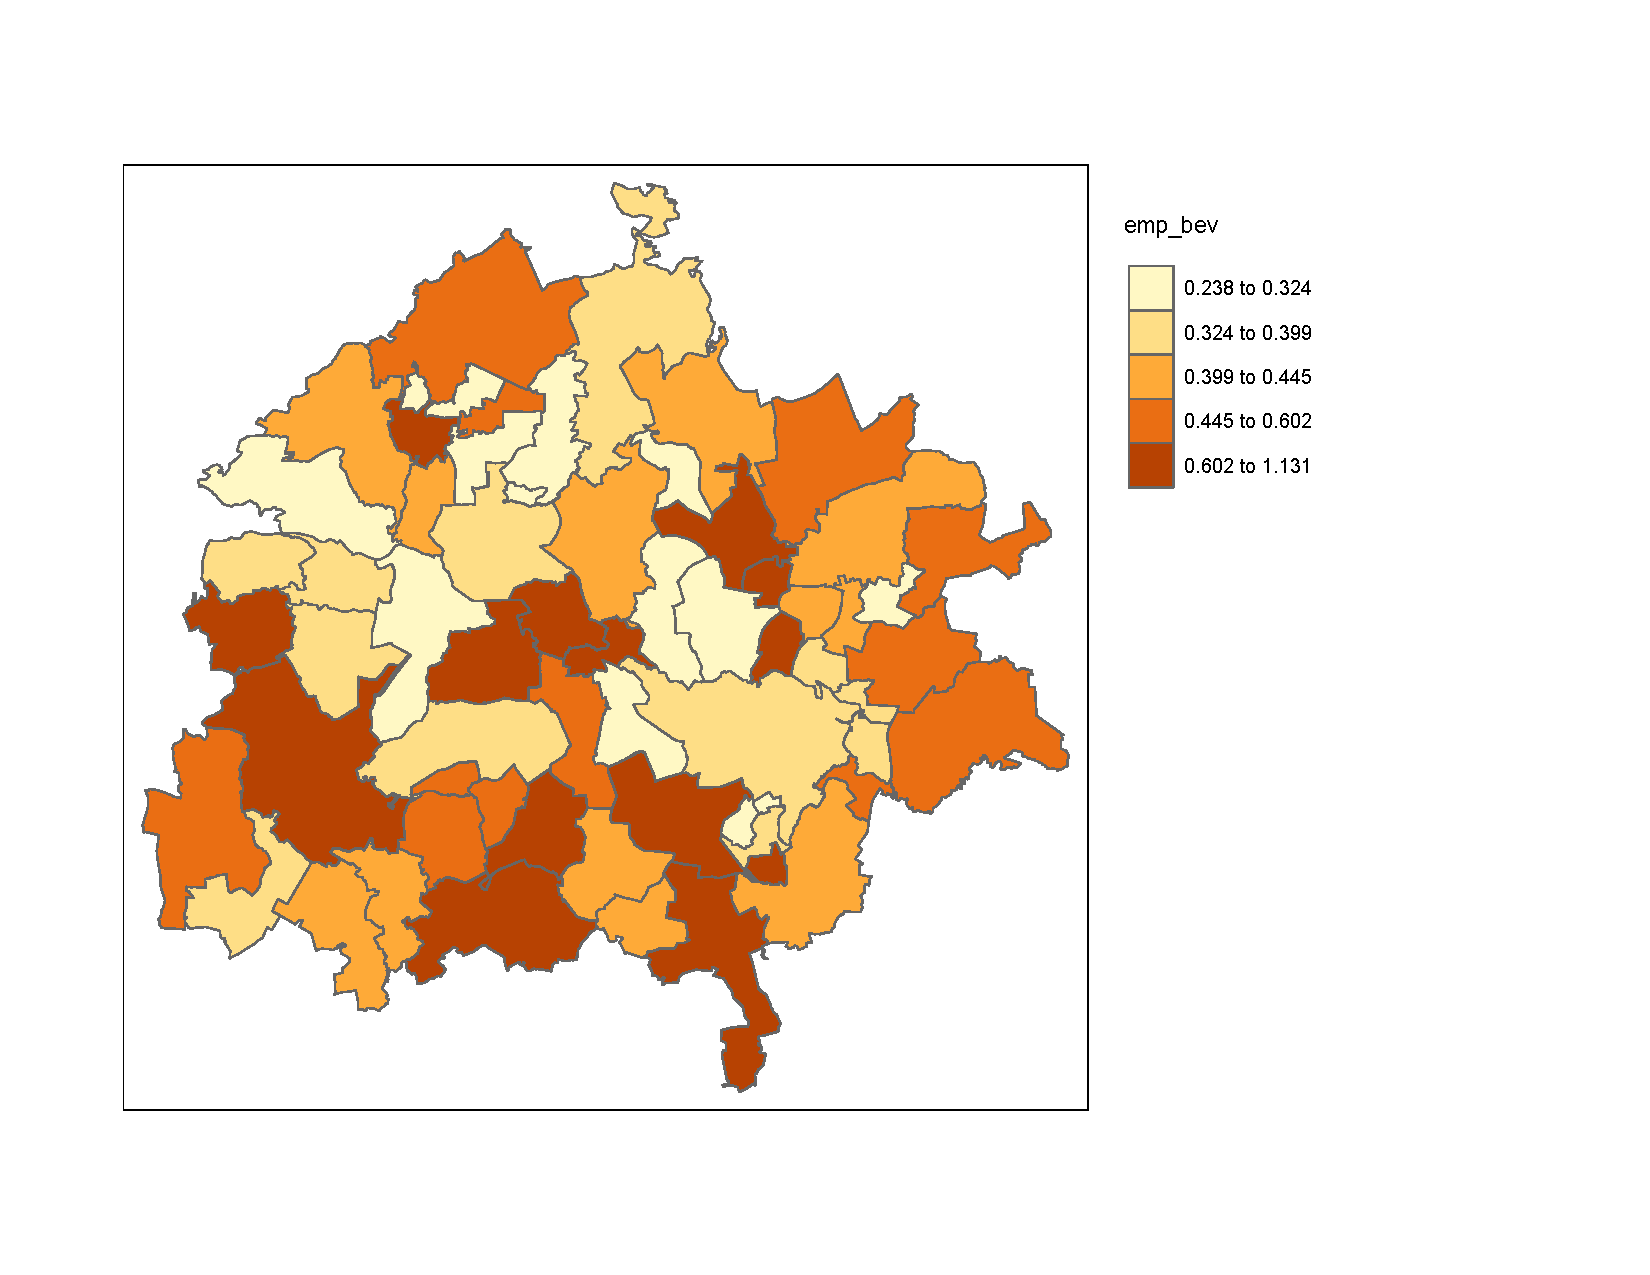
\includegraphics[scale=0.5,trim={2cm 2.7cm 5cm 2.7cm},clip]{body/figures/emp-bev.pdf}
                                   %trim={links unten rechts oben}    
    \end{center}
       %Source:
    \end{boxit}
    \caption[Quantilkarten]{Quantilkarten ausgesuchter Attribute in 2014. Grafik erstellt mit Daten aus: Quelle}
    \label{fig_quantilmaps}
\end{figure}


\begin{figure} %[htb] %h=here, t=top, b=bottom, p=page of float
    \centering %Bilder mittig statt am linken Rand ausgerichtet
    \begin{minipage}[b]{.45\linewidth} % [b] => Ausrichtung an \caption --> c (=Center) t (=Top) und b (=Bottom)
        % \linewidth entspricht hier \textwidth (=Breite Textbereich)
        %\centering
       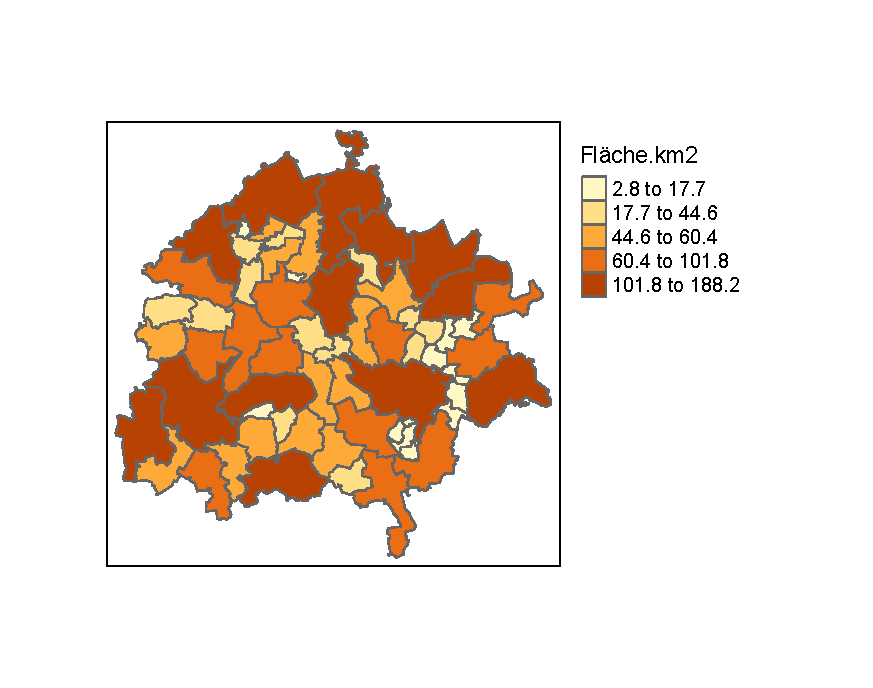
\includegraphics[scale=0.7,trim={1cm 2cm 1cm 2cm},clip]{body/figures/Rplot.pdf} % [scale=0.5] oder [width=\linewidth]
       %[width=\textwidth] entspricht [width=\linewidth] (=Breite einer Minipage)
       \caption{emp-bev}
    \end{minipage} % <- sonst wird hier ein Leerzeichen eingefügt
    \hfill
    %\hspace{.1\linewidth}% Abstand zwischen Bilder
    \begin{minipage}[b]{.45\linewidth}
        %\centering
       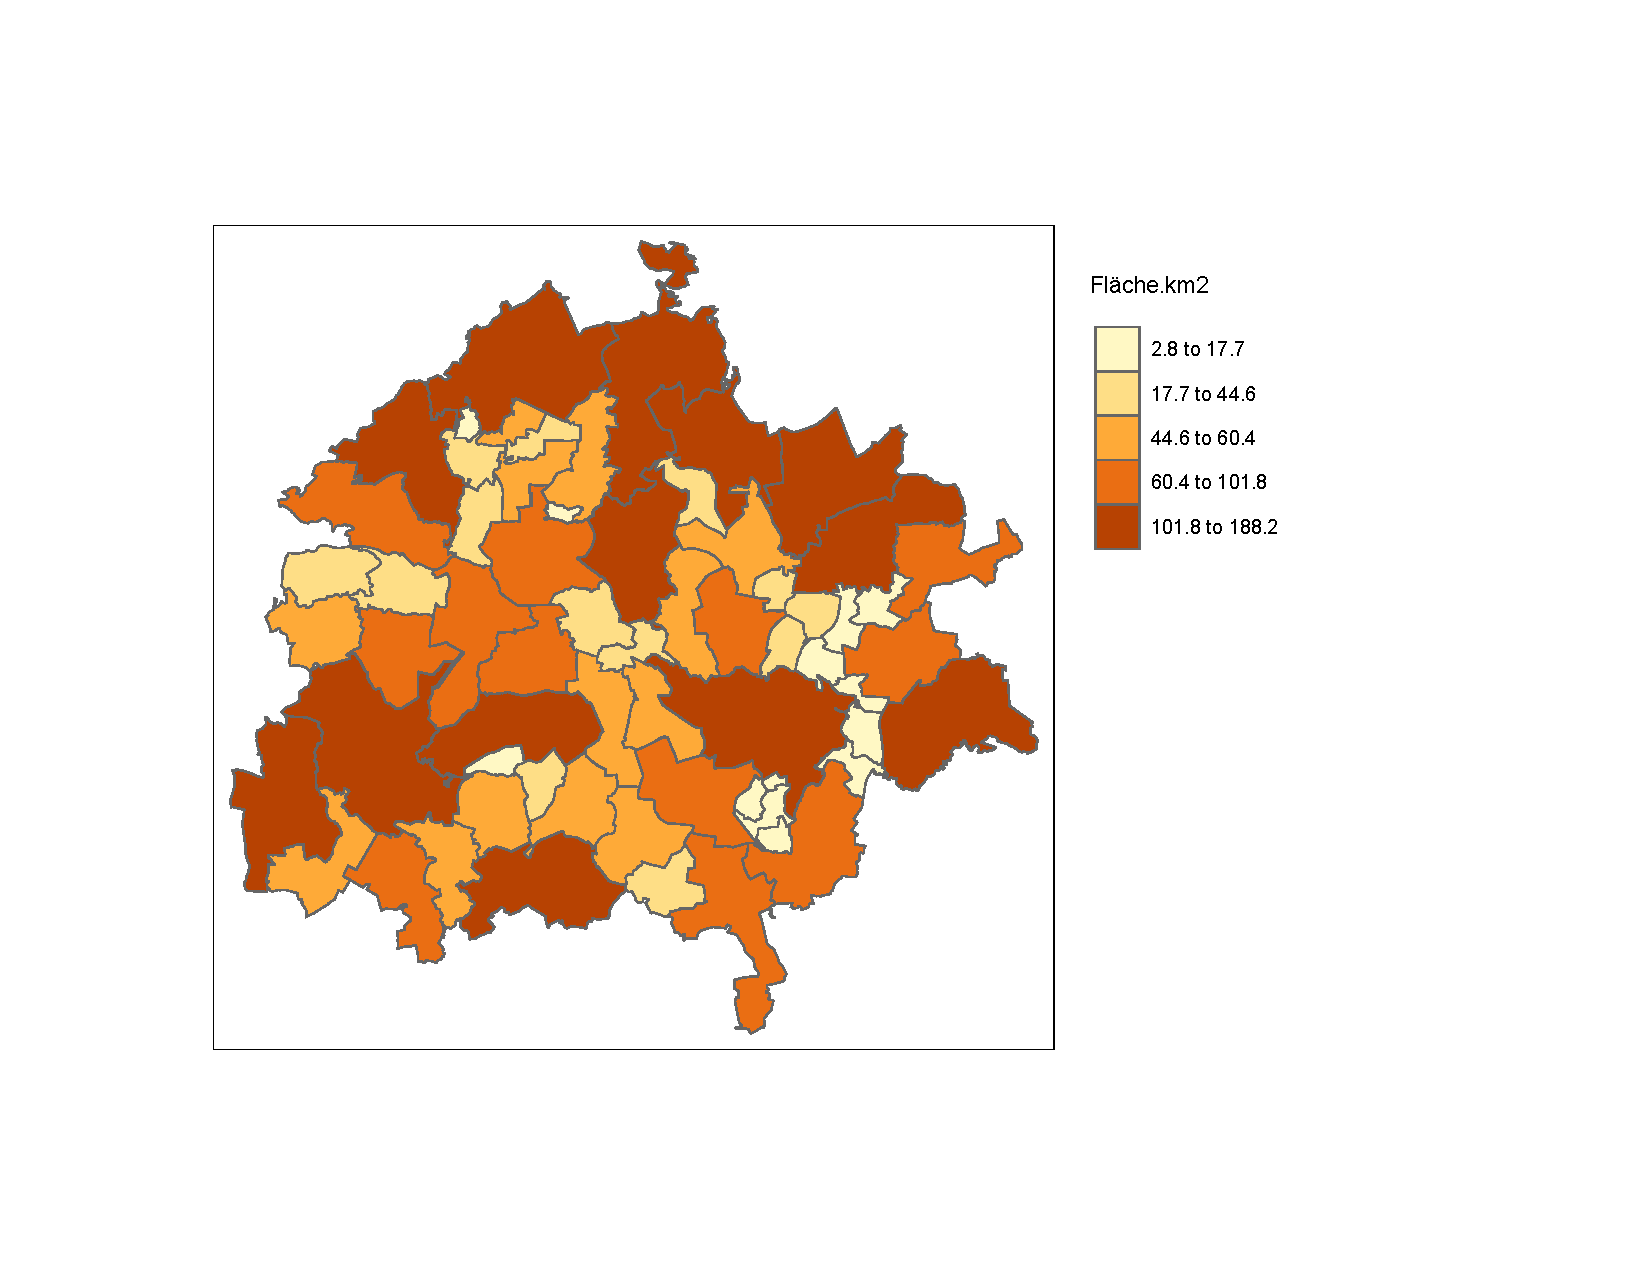
\includegraphics[width=\linewidth,trim={1cm 2cm 1cm 2cm},clip]{body/figures/km2.pdf}
       \caption{km2}
    \end{minipage}
 \end{figure}



\section{Lokaler Moran Index}
Je stärker der lokale Moran Index vom Erwartungswert abweicht und je größer der Z-Score bzw. je kleiner der p-Value sind, 
desto unwahrscheinlicher ist die Annahme von nicht autokorrelierten, zufallsverteilten Daten.


Zur detaillierten Untersuchung lokaler Autokorrelation eignet sich das Moran Scatterplot. 
Die Untersuchungsvariable  wird auf der x-Achse (Abszisse) dargestellt und die 
räumlich gewichteten, mittleren Nachbarwerte (engl. spatially lagged values) mittels y- Achse (Ordinate). 
Der globale Moran Index wird als linearer Zusammenhang zwischen beiden Dimensionen/Größen durch den Anstieg 
einer hervorgehobenen Geraden dargestellt. Der Plot wird zudem an Position der beiden 
Erwartungswerte in vier Quadranten zerlegt. Diese klassifizieren alle lokalen Beobachtungswerte 
entweder nach Clustern niedriger Werte (engl. Low-Low), nach Hot-Spots niedriger Werte(engl. Low-High), 
Hot-Spots hoher Werte (engl. High-Low) oder Clustern hoher Werte (engl. High-High).